\chapter{Donper}
\label{cap:donper}

\section{Introduzione}
\textbf{Donper} \cite{donper} è un fork di Damper \cite{damper}, che ne estende le funzionalità, implementando un funzionamento simile a HTB, seppur non uguale.\\ 
Nello specifico, è stata cambiata la struttura dati utilizzata dal precedente programma, per creare un albero \textbf{gerarchico} composta da un nodo padre con un numero variabili di nodi figli,
ognuno con una coda prioritaria di pacchetti e i parametri necessari. \\
Inoltre, è stata implementato pure un algoritmo di \textbf{prestito} di banda, simile a quello usato nella disciplina HTB.

\begin{figure}[!htb]
    \centering
    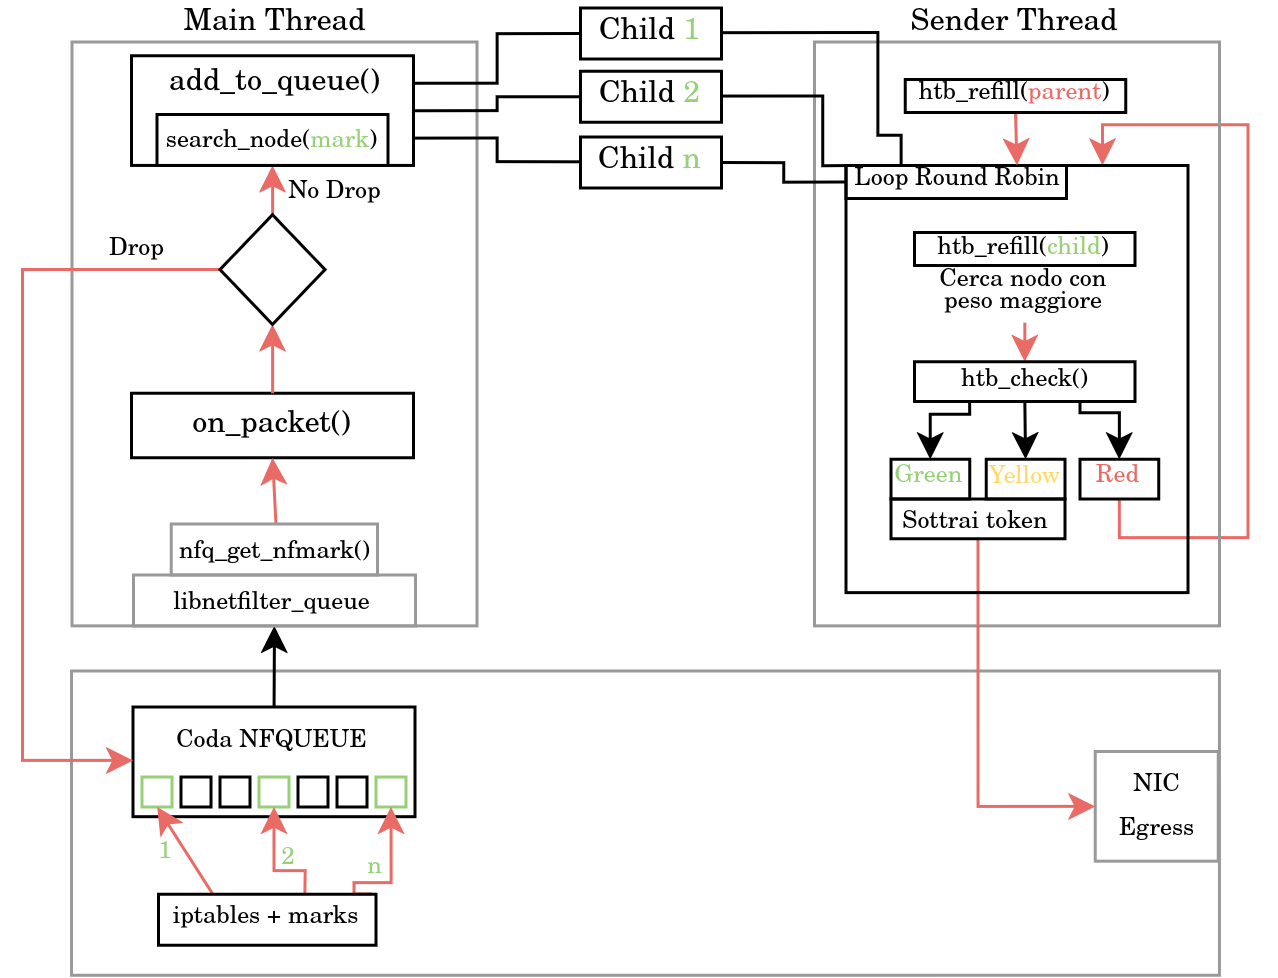
\includegraphics[width=0.8\linewidth]{Images/donper/donper.png}
    \caption{Architettura generale Donper.}
\end{figure}

Il programma modificato, come quello originale, mantiene due thread:
\begin{enumerate}
  \item \textbf{main thread:} si occupa del parsing del file di configurazione, della creazione dei nodi dell'albero e della gestione e classificazione dei pacchetti.
  \item \textbf{sender thread:} si occupa dell'invio dei pacchetti, utilizzando l'algoritmo token bucket e se necessario gestisce i prestiti fra nodi.
\end{enumerate}

Nelle prossime sezioni, verrà descritta l'implementazione in modo dettagliato, dimostiando fattibilità e limiti di questa nuova soluzione.

\section{Configurazione dei Parametri}
La configurazione dei parametri di ogni classe è possibile tramite il file \texttt{donper.conf}:

\begin{donper}[donper.conf]
# nfqueue queue id
queue 3

# traffic limit in bits per second (suffixes K, M and G allowed) for parent node
limit 40M
# bucket size for parent node in bytes
burst 50K

# htb
htb yes

# htb classes, limit >= sum(classes rates)
class mark 1 rate 20m ceil 40m burst 20k
class mark 2 rate 20m ceil 40m burst 20k
#class mark 3 rate 5m  ceil 10m burst 10k
#class mark 4 rate 5m  ceil 10m burst 10k

# modules
# number of recent flows
inhibit_big_flows nrecent 10
# dump debug info every 5 seconds
#inhibit_big_flows debug 5

# entropy module
entropy nrecent 10
#entropy debug 5
entropy k 2.0
# you can override source or destination port for this module
#entropy sport 0
#entropy dport 0
\end{donper}

Dall'implementazione orginiale, è stata aggiunta la possibilità di decidere se usare le classi e il prestito con il parametro \texttt{htb}.
Inoltre, è possibile configurare ogni classe con i suoi parametri principali:
\begin{itemize}
\item \textbf{Class Mark:} usato per definire la classe, il mark è possibile inserirlo tramite il comando \texttt{iptables}.
\item \textbf{Rate:} velocità di generazione dei token garantita.
\item \textbf{Ceil:} velocità massima possibile di generezione dei token.
\item \textbf{Burst:} capienza del bucket della classe.
\end{itemize}
Anche la configurazione del nodo padre richiede due parametri: \textbf{limit} (rate) e \textbf{burst}. \\
\vspace*{0.01\textheight}
La parte riguardante i moduli di assegnamento delle priorità ai pacchetti nell'array in user space, è stata mantenuta uguale.
Rimuovendo, però, la possibilità di usare i mark per assegnare i pesi.

\subsection{Struttura Dati}
Il cambio della strttura del file di configurazione, ha richiesto due grandi cambiamenti.
Il primo è la modifica della funzione \texttt{read\_config()}, per fare il parsing.
Il secondo, invece, è la creazione di due nuove strutture dati per la gestione dei parametri: 
\begin{enumerate}
  \item \texttt{Struct htb\_parent}: utilizzata per gestire i parametri del nodo padre.
  \item \texttt{Struct htb\_child}: rappresenta ogni nodo figlio, gestisce i parametri e l'array di pacchetti.
\end{enumerate}

\begin{clang}[Struct htb\_parent]
struct htb_parent {
    int queue;                /* nfequeue queue id */
    struct nfq_q_handle *qh;  /* queue handle */
    int nfqlen;               /* internal queue length */

    uint64_t limit;   /* or rate, bit/s */
    int64_t tokens;   /* token = byte */
    int64_t burst;    /* bucket size */

    struct timespec old_time;  /* old time to generate new tokens */

    pthread_t sender_tid;
    pthread_mutex_t lock;

    int htb;                       /* 1 for htb, 0 for tbf */
    struct htb_child **children;   /* array of the children */
    size_t n_children;             /* number of children node */
};
\end{clang}

All'interno, oltre i valori per lo shaping già elencati, sono contenuti pure:
\begin{itemize}
  \item I valori per gestire la NFQUEUE tramite \texttt{libnetfilter\_queue}, come l'id, l'handle e la lunghezza della coda.
  \item Tempo ultimo di refill dei token, usato per capire quanto tempo è passato dall'ultima volta che sono stati aggiunti gettoni.
  \item Pid del sender thread e mutex per gestire le risorse in modo sicuro.
  \item Array di nodi figli, con relativa lunghezza.
\end{itemize}

Invece, nella struttura dati di ogni nodo figlio:
\begin{clang}[Struct htb\_child]
struct htb_child {
    uint32_t mark;

    uint64_t rate;         /* min, byte/s */
    uint64_t ceil;         /* max with borrowing, byte/s */

    int64_t tokens;        /* number of token in the bucket */
    int64_t burst;         /* bucket size */
    int64_t ceil_tokens;   /* number of token for borrowing */
    int64_t ceil_burst;    /* burst for borrowing */

    struct timespec old_time;  /* old time to generate new tokens */
    struct timespec ceil_old_time; 

    /* priotirty queue */
    struct mpacket *packets;
    double *prioarray;
    size_t qlen;
};
\end{clang}
Oltre a tutti i valori per lo shaping è la divisione in classi, viene inserito pure un array di pacchetti, con i relatvivi persi e la lunghezza. \\
Utile notare che in questo caso, a differenza del padre, servono due tempi diversi per riempire il bucket, dato che si può riempire a due velocità diverse.
Infatti, deve essere gestito sia il caso in un cui non ci sia il prestito, con \texttt{rate}, \texttt{burst} e \texttt{tokens}, che il caso in cui ci sia, con \texttt{ceil}, \texttt{ceil\_burst} e \texttt{ceil\_tokens}.

\section{Classificazione dei Pacchetti}
Nello scorso capitolo, è stato accennato come per classificare i pacchetti nelle varie code, venga usato il valore \texttt{mark}. \\
Netfilter \cite{netfilter}, tramite il comando \texttt{iptables}, permette di inserire un valore da 32 bit nei paccheti di rete nel kernel space.
Questo permette di poter classificare i pacchetti tramite il numero assegnato, simulando il comportamento del parametro \texttt{class id} nella disciplina di coda HTB.
\vspace*{0.01\textheight}
In Donper, chi si occupa di questa situazione è la funzione \texttt{on\_packet()}:

\begin{clang}[Parte della funzione on\_packet()]
  mark = nfq_get_nfmark(nfad);

  pthread_mutex_lock(&parent->lock);
  if (weight < 0) {
    /* drop packet with with negative weight */
    nfq_set_verdict(parent->qh, id, NF_DROP, 0, NULL);
  } else {
    /* add to queue with positive weight */
    add_to_queue(parent, p, id, plen, weight, mark);
  }
  pthread_mutex_unlock(&parent->lock);
\end{clang}
Nello specifico, tramite la funzione \texttt{nfq\_get\_nfmark()}, salva il valore del mark del pacchetto e dopo aver controllato la positività del peso, chiama la funzione \texttt{add\_to\_queue()}.
Queste operazioni vengono eseguite in modo sicuro tramite il \texttt{pthread\_mutex}, per evitare una race condition fra thread. \\
\vspace*{0.01\textheight}
Successivamente, all'interno della funzione \texttt{add\_to\_queue()}, la variabile \texttt{mark}, verrò usata per cercare la classe corretta fra i vari nodi figli, tramite la funzione \texttt{search\_node()}:
\begin{clang}[Funzione search\_node()]
static int
search_node(struct htb_parent *parent, uint32_t mark)
{
  int i;
  
  if (!parent->htb) {
    return 0;
  }

  for (i=0; i<parent->n_children; i++) {
    if (parent->children[i]->mark == mark)
      return i;
  }

  return -1;
}
\end{clang}
Nel caso, sia stato scelto nel file di configurazione di non voler usare le classi, il valore di ritorno sarà sempre 0.\\ 
\vspace*{0.01\textheight}
Il funzionamento principale della funzione \texttt{add\_to\_queue()}, avendo il nodo corretto, è pressochè uguale a Damper. 
Si occuperà, quindi, di aggiungere il pacchetto all'array, sostituendolo, se necessario, con quello con peso minore.

\newpage
\section{Gestione della Trasmissione di Pacchetti}
Le funzioni delle sezioni precdenti erano gestite nel \textbf{thread principale}, invece, l'invio dei pacchetti, con il relativo shaping, deve essere fatto nel \textbf{sender thread}. \\ 
Inoltre, a differenza di Damper, il fork Donper deve essere in grado di gestire le diverse modalità, ossia con classi e prestito o senza.

\subsection{Prestito fra classi}
Per gestire il prestito fra classi, è necessario evidenziare le tre situazioni possibili in cui un nodo si può trovare:
\begin{enumerate}
  \item \textbf{GREEN:} il numero di tokens è sufficiente per inviare immediatamente il pacchetto.
  \item \textbf{YELLOW:} il numero di tokens non è sufficiente per inviare immediatamente un pacchetto, ma è possibile chiedere un prestito alla classe genitore, visto che la banda non è satura.
  \item \textbf{RED:} il numero di tokens non è sufficiente per inviare immediatamente un pacchetto e non è possibile prendere in prestito ulteriore banda. Il paccheto rimane in coda finchè non sarà possibile spedirlo.
\end{enumerate}
Nel programma questi tre casi sono descritti da:
\begin{clang}[enum htb\_mode]
enum htb_mode
{
  RED = 0,
  GREEN,
  YELLOW
};
\end{clang}
E gestiti dalla funzione \texttt{htb\_check()}, che controllando il numero di tokens disponibili della classe, ritorna uno di questi tre valori:
\begin{clang}[htb\_check()]
static enum htb_mode
htb_check(struct htb_parent *parent, struct htb_child *child, int64_t size)
{
  if ((child->tokens >= size)) {
    return GREEN;
  }

  if ((parent->limit != UINT64_MAX) && (parent->tokens < size)) {
    return RED;
  }

  if (child->ceil_tokens >= size) {
    return YELLOW;
  }

  return RED;
}
\end{clang}
\newpage

Invece, la condivisione di banda fra nodi figli è gestita automaticamente dalla logica del sender thread:
\begin{clang}[Parte della funzione sender\_thread()]
mode = htb_check(parent, child, size);
if (mode == RED) {
  /* no send */
  continue;
}

vres = nfq_set_verdict(parent->qh, child->packets[idx].id, NF_ACCEPT, 0, NULL);
if (vres < 0) {
  fprintf(stderr, "nfq_set_verdict() failed, %s\n", strerror(errno));
}

child->tokens -= size;
parent->tokens -= size;
if (mode == YELLOW) {
  child->ceil_tokens -= size;
}
\end{clang}
Nello specifico, per ogni classe, viene controllato il valore ritornato da \texttt{htb\_check()}. \\
Nel caso sia \textbf{RED}, viene usato l'istruzione \texttt{continue} per andare al nodo successivo, visto che non è possibile inviare.
Altrimenti, viene inviato alla NFQUEUE nel kernel il verdetto \texttt{NF\_ACCEPT}, tramite la funzione \texttt{nfq\_set\_verdict()}.
Per ogni pacchetto, deve essere sempre essere rimossa la dimensione del pacchetto da il valore \texttt{tokens} del nodo padre e del nodo figlio attuale,
invece, se il valore di ritorno è \textbf{YELLOW}, deve essere, pure, rimossa al valore \texttt{ceil\_tokens} del nodo figlio corrente.
\vspace*{0.01\textheight}
I tokens di ogni nodo devono essere, però, generati secondo il loro valore di rate/ceil. 
Per questo, è stata creata una funzione \texttt{htb\_refill()}, che funzioni sia per il nodo padre che per tutti i nodi figli:
\begin{clang}[Parte della funzione htb\_refill()]
clock_gettime(CLOCK_MONOTONIC, &now);

/* time passed in nano second */
ns = (now.tv_sec - old_time->tv_sec) * (int64_t)BILLION + (now.tv_nsec - old_time->tv_nsec);
if (ns <= 0) {
	return;
}

/* token generated */
add = (ns / (int64_t)BILLION) * (int64_t)rate + ((ns % (int64_t)BILLION) * (int64_t)rate) / (int64_t)BILLION;

*old_time = now;
\end{clang}
I token vengono generati usando i parametri \texttt{old\_time} \texttt{rate}/\texttt{ceil} del nodo passato.
Per prima cosa, viene calcolato il tempo passato dall'ultima volta che è stata chiamata la funzione \texttt{htb\_refill()}, successivamente viene trovato il valore corretto di tokens da aggiungere, tramite la formula:
\[
  \text{n\_tokens} = \text{time\_passed} \times \text{rate/ceil}
\]
Nel codice, non potendo usare valori decimali, è stata usata una forumla per aggiungere pure il resto corretto, visto che il casting a un intero avrebbe fatto perdere precisione.\\ 
Infine, viene aggiornata la variabile \texttt{old\_time}, per il prossimo uso.

\subsection{Gestione senza Classi}
Una modalità di utilizzo di Donper prevede il funzionamento anche senza classi, simulando la disciplina di coda TBF, visto che nel programma precedente Damper era implementato in modo diverso. \\
\vspace*{0.01\textheight}
Tramite il file di configurazione \texttt{donper.conf} è possibile decidere con il parametro \texttt{htb} di voler utilizzare questa modalità. \\ 
In questo caso, nell funzione di inizializzazione delle strtture dati \texttt{tree\_init()}:
\begin{clang}[Parte di tree\_init()]
/* no class or no htb, then tbf */
if (parent->n_children == 0) {
  parent->n_children += 1;

  /* using one child node for tbf */
  parent->children[0] = malloc(sizeof(struct htb_child));
  if (!parent->children[0]) {
		  fprintf(stderr, "malloc(%lu) failed\n", (long)sizeof(struct htb_child));
		  goto fail_conf;
}

  /* using parent value */
  parent->children[0]->rate = parent->limit;
  parent->children[0]->ceil = parent->limit;
  parent->children[0]->burst = parent->burst;
  parent->children[0]->ceil_burst = parent->burst;
}
\end{clang}
Nel pratico, viene creato una sola classe, con gli stessi valori del nodo padre, per gestire l'unica coda di pacchetti che servirà.\\ 
Il motivo di questa scelta è che le funzioni elencate nella sezione prima funzionano solo sui nodi figli, quindi in questo modo non è stato necessario cambiare o aggiungere codice in più.

\section{Verifica Sperimentale}
Per verificare il funzionamento del programma, verrà riproposto l'esercizio \ref{sec:htb}.
\begin{note}[Scenario]
  Un server di un'azienda ospita tre servizi per tre clienti diversi: un servizio streaming, un sito web con molto traffico e un servizio di file hosting. \\ 
  La banda totale disponibile e garantita è 100 Mbit/s. Si vuole garantire più banda al cliente del sito web rispetto agli altri due clienti.
  Gli altri due servizi avranno un minimo di banda garantita.
\end{note}

\begin{figure}[!htb]
    \centering
    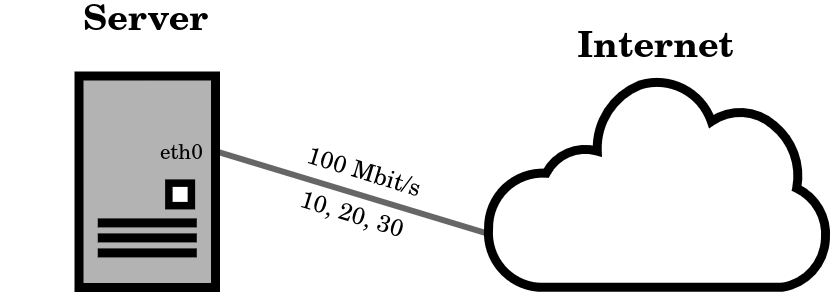
\includegraphics[width=0.6\linewidth]{Images/donper/scenario.png}
    \caption{Rappresentazione grafica scenario.}
\end{figure}

In questo caso, non sarà possibile usare i class id, ma dovranno essere usati tre mark diversi: \textbf{10}, \textbf{20} e \textbf{30}.

\subsection{Soluzione}
Come ambiente di simulazione verra usato Kathará, dove saranno presenti quattro nodi diversi: uno per simulare il server e tre per simulare i clienti.
La parte riguardante l'impostazione dei file \texttt{lab.conf} e \texttt{pc<n>.startup} verrà omessa, dato che sarebbe uguale a quelle già viste. \\ 
\vspace*{0.01\textheight}
Per prima cosa, è necessario chiarire come usare il comando \texttt{iptables} con questo nuovo programma. 
Non sarà più necessario solo intercettare il traffico e matterlo in una coda NFQUEUE in kernel space, ma per ogni paccheto dovrà essere pure assegnato un mark:
\begin{bash}[Regole iptables]
# Mark 10
iptables -t mangle -A OUTPUT -p tcp --sport 80  -j MARK --set-mark 10
iptables -t mangle -A OUTPUT -p tcp --sport 443 -j MARK --set-mark 10

# Mark 20
iptables -t mangle -A OUTPUT -p tcp --sport 554 -j MARK --set-mark 20

# Mark 30
iptables -t mangle -A OUTPUT -p tcp --sport 21  -j MARK --set-mark 30

# NFQUEUE
iptables -t mangle -A OUTPUT -j NFQUEUE --queue-num 0 --queue-bypass
\end{bash}
Inoltre, non sarà più possibile usare la tabella \textbf{raw}, altrimenti non verrebbe letto il mark, quindi la soluzione naturale è usare la tabella \textbf{mangle}.
\vspace*{0.01\textheight}
Successivamente, dovrà essere modificato il file \texttt{donper.conf} in modo coerente allo scenario e alle regole:
\begin{donper}[donper.conf]
# nfqueue queue id
queue 0

# traffic limit in bits per second (suffixes K, M and G allowed) per il nodo padre
limit 100M

# bucket size parent node
burst 20K

htb yes

# classes
class mark 10 rate 50m ceil 100m burst 10k
class mark 20 rate 35m ceil 60m burst 7k
class mark 30 rate 15m ceil 20m burst 4k
\end{donper}
Infine, avviando Donper con il relativo file, sarà possibile valutare i tempi.
\begin{bash}[Avvio di Donper]
donper /etc/donper/donper.conf &
\end{bash}

\newpage
\subsection{Risultati}
Dopo aver creato un file da 100 MB:
\begin{bash}
dd if=/Dev/urandom of=file.bin bs=100M count=1
\end{bash}
Si possono valutare i tempi con il comando \texttt{nc} come negli esercizi degli altri capitoli. \\
Per vedere il corretto funzionamento del programma, vanno verificate tre situazioni diverse:
\begin{enumerate}
  \item Tutti i nodi comunicano con il server contemporaneamente.
  \item Solo due nodi comunicano con il server contemporaneamente.
  \item Solo un nodo comunica con il server contemporaneamente.
\end{enumerate}

Per prima cosa è necessario capire i tempi ideali da confrontare:
\begin{center}
  \begin{tabular}{ |>{\columncolor{gray!35}}c|c|c| }
    \hline
    \rowcolor{gray!35}
    $\space$ & \textbf{Ideale per Rate} & \textbf{Ideale per Ceil} \\
    \hline
    \textbf{Client 1} & 16.00s & 8.00s \\
    \hline
    \textbf{Client 2} & 22.86s & 13.33s \\
    \hline
    \textbf{Client 3} & 53.33s & 40.00s \\
    \hline
  \end{tabular}
\end{center}
Successivamente, con le stesse modalità degli esercizi dei capitoli scorsi, si possono calcolare i tempi del programma Donper:
\begin{figure}[htbp]
  \centering
  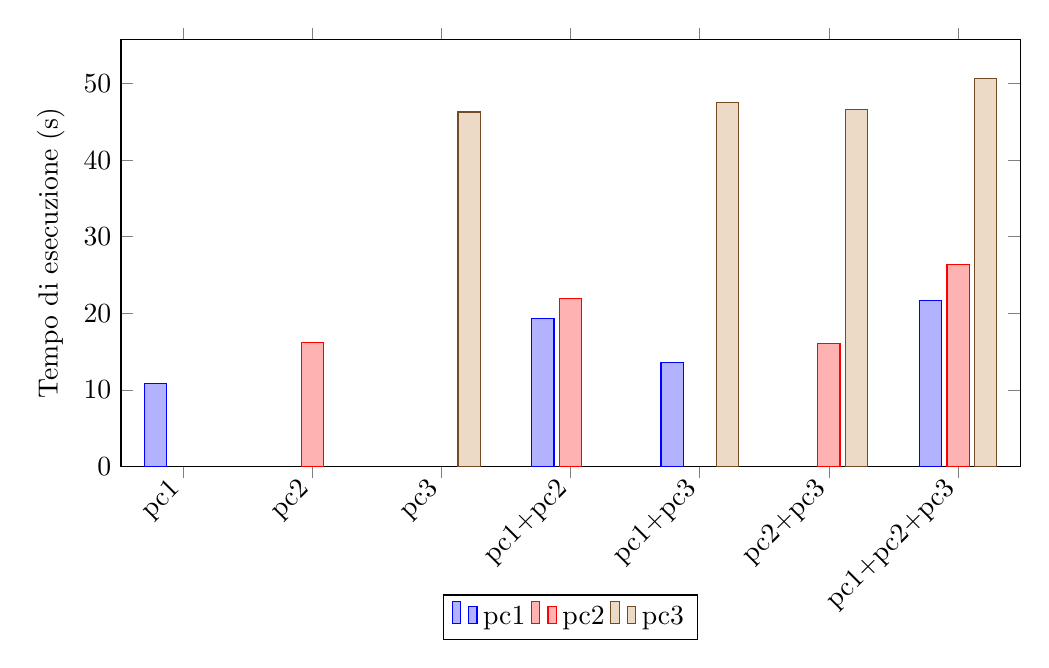
\begin{tikzpicture}
    \begin{axis}[
        ybar,
        bar width=8pt,
        width=13cm,
        height=7cm,
        ylabel={Tempo di esecuzione (s)},
        symbolic x coords={pc1, pc2, pc3, pc1+pc2, pc1+pc3, pc2+pc3, pc1+pc2+pc3},
        xtick={pc1, pc2, pc3, pc1+pc2, pc1+pc3, pc2+pc3, pc1+pc2+pc3},
        x tick label style={rotate=45, anchor=east},
        ymin=0,
        enlarge x limits=0.08,
        legend style={at={(0.5,-0.3)}, anchor=north, legend columns=-1},
        ]
      % Tempo di pc1 nelle configurazioni in cui pc1 è attivo
      \addplot coordinates {
        (pc1, 10.808)
        (pc1+pc2, 19.340)
        (pc1+pc3, 13.560)
        (pc1+pc2+pc3, 21.619)
      };
      % Tempo di pc2 nelle configurazioni in cui pc2 è attivo
      \addplot coordinates {
        (pc2, 16.145)
        (pc1+pc2, 21.972)
        (pc2+pc3, 16.028)
        (pc1+pc2+pc3, 26.418)
      };
      % Tempo di pc3 nelle configurazioni in cui pc3 è attivo
      \addplot coordinates {
        (pc3, 46.284)
        (pc1+pc3, 47.550)
        (pc2+pc3, 46.555)
        (pc1+pc2+pc3, 50.647)
      };
      \legend{pc1, pc2, pc3}
    \end{axis}
  \end{tikzpicture}
\end{figure}

I tempi misurati si avvicinano a quelli ideali con velocità ceil quando gli altri client sono assenti, e a quelli con velocità rate quando tutti e tre sono attivi.

\section{Considerazioni Finali}
I risultati ottenuti confermano che Donper riesce a riprodurre, in userspace, un comportamento simile a quelli di HTB e TBF. 
I tempi calcolati rispettano il rate garantito nel caso in cui i nodi siano tutti attivi e il ceil nel caso sia possibile il prestito, aggiungendo un overhead accettabile di circa 1,5/2 secondi. \\
\vspace*{0.01\textheight}
L'introduzione di una struttura gerarchica, unita all'utilizzo dell'algoritmo token bucket, risolve i principali limiti di Damper spiegati nella sezione \ref{sec:limiti}.
La possibilità di gestire più flussi tramite un solo file, senza dover usare più istanze del programma, rende anche più semplice la gestione di più classi.
